\documentclass[conference]{IEEEtran}
\IEEEoverridecommandlockouts
\usepackage{amsmath,amssymb,booktabs,multirow,graphicx,url,xcolor}
\usepackage[hidelinks]{hyperref}
\usepackage{algorithm}
\usepackage{algpseudocode}
\usepackage{balance}

\title{Beyond Bigger Models and Longer Contexts: Resource--Quality Frontiers for Portable LLM-Agent Extraction}

\author{
\IEEEauthorblockN{Manal Helal}
\IEEEauthorblockA{
School of Physics, Engineering and Computer Science\\
University of Hertfordshire\\
Hatfield, United Kingdom\\
m.helal@herts.ac.uk
}
}
\begin{document}
\maketitle

\begin{abstract}
Production LLM agents are assembled from hosted and local models, retrieval, validation, retries and concurrent tool calls, yet deployment choices are still often based on nominal context length or parameter count. This paper studies the resulting \emph{resource--quality frontier} for source-grounded extraction agents. We analyse 136 attempted runs (111 successful, 25 unsuccessful) comprising 1{,}689 realised model calls across seven campaigns varying extraction partition size, model/role assignment, fan-out concurrency and critic depth, preserving campaign identity rather than pooling heterogeneous serving conditions. Three results recur. First, context is non-monotonic: 14k-character partitions give the strongest source-grounded fidelity in both partitioning campaigns and the lowest cost per verified claim in the failure-free one, 6k partitions favour raw extraction quantity, while 28k partitions collapse to zero verbatim fidelity despite the lowest wall time. Second, two-way fan-out achieves the lowest observed mean latency in two campaigns run on two different serving substrates---a hosted OpenAI-compatible endpoint and a local single-user runtime---while four-way fan-out reverses part or all of the gain. Third, nominal parameter count is not a sufficient capacity proxy: a general-purpose 8B model was 7.32$\times$ faster than a 70B model and 12.77$\times$ more efficient per verified claim, a 31B model achieved higher fidelity than a 550B/A55B endpoint, and a safety-specialised 8B endpoint returned syntactically valid JSON conforming to its own classification schema rather than the requested extraction schema, failing every attempt. We extend a prior communication--computation ratio (CCR) into a prefill/decode-aware optimisation model and propose a provider-neutral campaign schema recording realised provider/model identity, failures, output validation and serving metadata. The results motivate workload-specific partitioning, bounded concurrency, capability-aware routing, and standardised inference telemetry rather than provider- or model-size-specific tuning.
\end{abstract}

\begin{IEEEkeywords}
LLM agents, inference serving, context partitioning, prefill, decode, concurrency, interoperability, reproducibility, resource--quality optimisation
\end{IEEEkeywords}

\section{Introduction}
Large language model (LLM) applications are no longer single-model programs. Production systems combine prompts, retrieval, multiple model roles, structured-output validation, retries, routing and serving infrastructure. This shifts the engineering question from ``which model is best?'' to \emph{which operating point delivers sufficient task quality at acceptable latency, throughput and deployment cost?} The distinction matters because model quality measured in isolation does not determine system quality; configuration, serving, dependencies and external state contribute substantial operational complexity \cite{sculley2015debt}.

LLM serving sharpens the problem. Autoregressive inference has two operationally distinct phases: \emph{prefill}, which processes the input and determines time-to-first-token (TTFT), and \emph{decode}, which generates output tokens sequentially and determines inter-token latency (ITL) and time per output token (TPOT). Recent serving work disaggregates them because they have different resource characteristics \cite{zhong2024distserve}, and MLPerf evaluates server-mode inference using TTFT and TPOT rather than one undifferentiated latency \cite{mlperf2025llm}. Long context is consequently not ``free'': input length drives prefill and KV-cache pressure, while output length drives repeated decode work. NVIDIA's sizing guidance likewise treats sequence lengths, TTFT, ITL and concurrency as joint deployment variables \cite{nvidiaRAGSizing,nvidiaDynamoProfiler}.

Agent pipelines add a second source of complexity: the logical pipeline and the realised serving path need not be identical. APIs may be syntactically compatible while differing in model catalogues, structured-output behaviour, retry semantics, token accounting, queueing and exposed performance telemetry. An application may also route among hosted and local providers, automatically and mid-run. An experiment must therefore record not only the configured model but the \emph{realised} provider/model for every call. This is a systems interoperability issue rather than an exceptional condition: portable agent software requires a stable contract above provider-specific serving behaviour.

This paper positions extraction-agent design as a resource--quality optimisation problem. Prior distributed-computing work selected partition size by balancing communication and computation using a communication--computation ratio (CCR) \cite{helal2008parallel,helal2009search,helal2009thesis}. The same principle transfers naturally to LLM agents, but the ``work'' term must now distinguish prefill from decode and accommodate queueing/serving state.

The contributions are:
\begin{itemize}
\item a cross-campaign empirical characterisation comprising seven campaigns, 136 attempted runs and 1{,}689 realised model calls, retaining every operating point rather than discarding results when model catalogues evolve;
\item replicated evidence that context size and concurrency exhibit non-monotonic resource--quality frontiers, and that nominal model size alone does not predict extraction utility;
\item a prefill/decode-aware CCR model that connects partition selection to input length, generated length, fixed invocation cost and serving variation, demonstrated on measured operating points;
\item a provider-neutral experiment and attribution schema for merging heterogeneous campaigns without erasing model/provider identity; and
\item deployment recommendations for capability-aware routing, bounded fan-out, realised-call provenance, and standardised serving telemetry.
\end{itemize}

\section{Research Positioning}
\subsection{Serving optimisation and the missing application-level frontier}
Production serving designs increasingly optimise requests jointly rather than in isolation. Orca introduced iteration-level scheduling so requests join and leave a running batch between decoding steps \cite{yu2022orca}; vLLM adds PagedAttention to reduce KV-cache fragmentation and raise batch size \cite{kwon2023vllm}; SGLang adds RadixAttention for prefix/KV reuse in structured multi-call programs, a common agent pattern \cite{zheng2024sglang}; Sarathi-Serve chunks prefills to control the throughput--latency trade-off \cite{agrawal2024sarathi}; TensorRT-LLM supplies optimised kernels, in-flight batching and paged KV caching \cite{nvidiaTensorRTLLM}; and DistServe separates prefill from decode to optimise TTFT and TPOT under service objectives \cite{zhong2024distserve}. They differ in mechanism but share a premise: concurrent requests should be co-scheduled with awareness of KV state, batching and generation progress.

This serving literature primarily optimises the engine. Our concern is complementary: an \emph{agent application} changes the workload presented to that engine by changing partition size, model/role assignment, fan-out and validation depth. Long-context benchmarks demonstrate capability at large sequence lengths, but maximum supported context is not necessarily the best application partition. MLPerf now evaluates long-context LLM server performance with TTFT/TPOT constraints \cite{mlperf2025llm}; our question is the application-level analogue: when a source can be partitioned, which context regime maximises verified task output per unit resource?

\subsection{Hosted, local and agent-generated concurrency}
Local interactive runtimes and throughput-oriented serving stacks embody different concurrency assumptions. Ollama prioritises lightweight local use and bounded parallel request slots, whereas vLLM is designed for dynamically batched high-concurrency serving. In a controlled Red Hat comparison using matched Llama-3.1-8B weights on the same A100, vLLM achieved higher throughput and lower tail latency across the tested concurrency range even after Ollama's parallel-request limit was raised to 32 \cite{redhat2025ollamavllm}. This distinction is especially relevant to agents: fan-out stages generate bursts of simultaneous requests by construction, so a client-side concurrency result measured on one serving design should not be assumed to transfer unchanged to another. We exploit this directly: our two fan-out campaigns were executed on two different substrates, allowing the concurrency finding to be tested rather than assumed portable.

\subsection{Interoperability beyond API syntax}
Standard interfaces reduce integration cost, as ONNX did between training frameworks and inference runtimes \cite{onnx2019}. LLM APIs have converged on OpenAI-like request/response shapes, and NIM exposes OpenAI-compatible APIs over optimised NVIDIA serving stacks \cite{nvidiaNIM}. Yet API compatibility does not imply execution-semantic compatibility: providers differ in catalogues, structured-output handling, token accounting, retry/fallback behaviour, batching, queueing and telemetry. Section~\ref{sec:models} reports a case in which a request succeeded at the HTTP and JSON levels and still returned an unusable object. Reproducible agent execution therefore needs a second interoperability layer---a common trace contract for realised provider/model identity, TTFT/ITL, queue and server time where available, output validation, retries and terminal status. We treat this \emph{observability interoperability} as a first-class requirement.

\section{CCR-Guided Resource--Quality Optimisation}
Prior distributed alignment work used partitioning to balance computation against communication, showing that partition structure can determine whether parallelism helps at all \cite{helal2008parallel,helal2009search}. Let the coarse latency model be
\begin{equation}
T(m) = t_s+t_w m,
\end{equation}
where $t_s$ is fixed start-up/communication cost, $t_w$ is work per unit, and $m$ is partition work. The corresponding ratio
\begin{equation}
CCR = \frac{t_s}{t_wm}
\label{eq:ccr-old}
\end{equation}
indicates whether fixed invocation/communication or useful work dominates.

For autoregressive LLM inference, a single work coefficient hides two different phases. We therefore use
\begin{equation}
T \approx t_s + t_p N_{in} + t_d N_{out} + \epsilon(h,c,p),
\label{eq:latency}
\end{equation}
where $N_{in}$ and $N_{out}$ are input and output tokens, $t_p$ is the prefill cost per input token, $t_d$ is the decode cost per output token, and $\epsilon$ captures hosted-service state $h$, concurrency $c$, provider/runtime $p$, network and queueing. Here $T$ is end-to-end application-observed latency, which may include client processing, network transfer, provider queueing, inference, validation and retries. In contrast, prefill and decode are internal inference phases. The coefficients $t_p$ and $t_d$ represent effective application-level cost components, not directly measured GPU kernel times. Without provider-side telemetry or controlled experiments, these components cannot be uniquely separated from queueing and other overheads. Equation~\ref{eq:latency} is therefore a proposed observable cost model, not an empirical decomposition of the reported wall-clock measurements. It yields
\begin{equation}
CCR_{PD} = \frac{t_s+\hat{\epsilon}}{t_pN_{in}+t_dN_{out}}.
\label{eq:ccr-pd}
\end{equation}
When only aggregate timing is exposed, $t_pN_{in}+t_dN_{out}$ can be collapsed to $t_wm$, recovering Eq.~\ref{eq:ccr-old}. When TTFT/ITL telemetry is available, $t_p$ and $t_d$ can be estimated separately. This mirrors contemporary serving practice, which models TTFT as prefill-sensitive and ITL/TPOT as decode-sensitive \cite{zhong2024distserve,nvidiaDynamoProfiler}.

CCR alone does not select the partition because extraction quality is non-monotonic. We therefore choose a partition $m^*$ from feasible candidates $\mathcal{M}$ by
\begin{equation}
m^*=\arg\min_{m\in\mathcal{M}} \frac{T(m)}{N_c(m)V(m)}
\quad \text{s.t.}\quad V(m)\ge V_{min},
\label{eq:utility}
\end{equation}
where $N_c$ is extracted claims and $V$ is source-grounded verbatim fidelity. The denominator $N_cV$ is the expected number of verbatim-grounded claims, making seconds per verified claim an interpretable resource--quality objective. CCR predicts whether finer partitioning will be dominated by invocation overhead; the quality constraint prevents selecting an apparently fast but semantically collapsed long-context regime.

The threshold $V_{\min}$ is an application requirement rather than a universal constant. It should be selected before configuration tuning, from the level of source-grounding the downstream task actually needs: a regulated evidence pipeline that must quote sources exactly demands a high $V_{\min}$, whereas an exploratory survey tool may accept a low one in exchange for breadth. Threshold sensitivity can then be assessed by repeating the feasible-set selection over several values of $V_{\min}$, without rerunning inference, because the candidate measurements are already available.

\subsection{A worked example on measured operating points}
\label{sec:worked}
Table~\ref{tab:ev} applies Eq.~\ref{eq:utility} to the nine measured cells of our first partitioning campaign, which completed all 27 attempts without failure and therefore needs no success filtering. Reading it top to bottom is the whole method in miniature.

\begin{table}[t]
\caption{Quality-constrained operating-point selection on measured cells (partitioning campaign~A; 3/3 successful runs in every cell). $E_v=T/(N_cV)$ is seconds per verbatim-grounded claim; lower is better.}
\label{tab:ev}
\centering\scriptsize
\begin{tabular}{rrrrrrr}
\toprule
Window & Workers & $T$ (s) & sd & $N_c$ & $V$ & $E_v$\\
\midrule
6k  & 1 & 680.4 & 181.2 & 50.7 & .510 & 26.33\\
6k  & 2 & 616.8 &  27.9 & 53.3 & .372 & 31.09\\
6k  & 4 & 597.5 & 201.4 & 48.0 & .371 & 33.55\\
14k & 1 & 469.8 & 294.0 & 28.3 & \textbf{.762} & \textbf{21.76}\\
14k & 2 & 569.0 & 415.3 & 24.7 & .731 & 31.55\\
14k & 4 & 577.3 & 105.2 & 31.7 & .709 & 25.71\\
28k & 1 &  66.3 &  39.7 &  4.0 & .000 & undef.\\
28k & 2 &  55.9 &  35.8 &  2.3 & .000 & undef.\\
28k & 4 &  80.4 &  19.2 &  4.7 & .000 & undef.\\
\bottomrule
\end{tabular}
\end{table}

Three readings follow. (i) \emph{Latency alone selects the worst configuration.} The three fastest cells are all 28k and all produce zero verbatim-grounded claims: $N_cV=0$, so $E_v$ is undefined and they are infeasible at any $V_{\min}>0$. A deployment tuned on wall time would choose exactly these. (ii) \emph{Quantity alone also misleads.} The 6k regime extracts the most claims, peaking at 53.3, but at roughly half the fidelity of 14k, so its best cell costs 26.33\,s per verified claim against 21.76\,s. (iii) \emph{The constraint changes the feasible set, not the winner here.} At $V_{\min}=0.50$ the feasible set is 6k/1 and all three 14k cells; at $V_{\min}=0.70$ only 14k survives; at either threshold 14k/1 minimises $E_v$. The threshold matters most when the objective is near-tied---the 14k/1 to 6k/1 gap is 17\%, so a workload valuing recall over grounding could reasonably prefer 6k.

Equation~\ref{eq:ccr-pd} explains \emph{why}. Halving the window from 14k to 6k roughly doubles the calls on this document (18.7 against 33.7 per run); each call re-pays $t_s$ and re-sends shared instruction context, so fixed cost rises while useful work per call falls---a rising $CCR_{PD}$. Widening to 28k reduces the document to two windows and 2.3 calls, minimising invocation overhead and wall time but reaching an operating point where the model no longer reproduces source text verbatim at all. CCR identifies the overhead- and work-dominated ends; the quality constraint rules out the degenerate end CCR alone would reward.

\section{Experimental Method}
\subsection{Campaign design}
We analyse seven separately recorded campaigns comprising 32 experimental conditions, 136 attempted runs and 1{,}689 realised model calls. Of the attempts, 111 completed successfully and 25 ended unsuccessfully. The experiments comprise repeated within-condition observations rather than 136 independent workload configurations; accordingly, the reported findings are interpreted as workload-specific operating points.

We retain campaign identity because hosted inference is a time-varying environment. A cell changes one experimental factor while holding the task and evaluation protocol fixed within that campaign. Each campaign remains a valid observation of the model/provider configuration available when it executed; later catalogue changes represent new operating conditions rather than grounds for removing earlier measurements. We refer throughout to \emph{earlier} and \emph{later} campaigns where the distinction is analytically relevant, and label campaigns A/B within each factor.

\begin{table}[t]
\caption{Cross-campaign experimental inventory.}
\label{tab:inventory}
\centering\scriptsize
\begin{tabular}{lrrrr}
\toprule
Campaign & Conditions & Attempts & Failures & Calls\\
\midrule
Partitioning A & 9 & 27 & 0 & 462\\
Partitioning B & 9 & 45 & 20 & 276\\
Role sizing A & 2 & 10 & 0 & 301\\
Role sizing B & 3 & 9 & 3 & 138\\
Fan-out A & 3 & 15 & 1 & 197\\
Fan-out B & 3 & 15 & 1 & 90\\
Protocol & 3 & 15 & 0 & 225\\
\midrule
Total & 32 & 136 & 25 & 1689\\
\bottomrule
\end{tabular}
\end{table}

Six campaigns run a citation-extraction agent over a 34{,}651-character source document; the protocol campaign runs a rubric-based assessment agent over a separate 21{,}871-character document, and is reported separately for that reason. The core metrics are end-to-end wall-clock time, claims extracted, references matched, verbatim fidelity $V$, resolution rate, pooled recall, corroboration and cross-run stability. Verbatim fidelity measures whether extracted claims satisfy a deterministic source-text matching criterion; it does not establish semantic correctness, entailment or completeness. A paraphrased but correct claim may fail verbatim matching, while a verbatim passage may still mislead out of context. Pooled recall is interpreted against the available reference set, not as exhaustive recall over the source. We additionally report
\begin{equation}
E_v=\frac{T}{N_cV},
\end{equation}
seconds per verbatim-grounded claim. Here $N_c$ is the number of extracted claims and $V\in[0,1]$ is the fraction satisfying the source-verbatim matching criterion, so $N_cV$ estimates the number of verbatim-grounded claims; it is not a manual semantic-correctness score. $E_v$ is undefined when $N_cV=0$ and is not assigned an artificial finite value.

An attempted run is unsuccessful when it terminates without producing a valid extraction result under the task-output contract. The 25 unsuccessful attempts resolve into five recorded causes: 19 preflight refusals, three runs in which every fan-out worker raised, and one each of no parseable window, a zero-claim guard, and a stage failure without a terminal record. The 19 refusals are a single event. Between 03:03 and 04:08 UTC on 31 August the configured deep endpoint began answering 404, and the harness declined to start any job whose configuration it could not satisfy. Those jobs issued no model call at all, which is why campaign~B records 45 attempts but only 276 realised calls against campaign~A's 27 attempts and 462 calls. The same endpoint served 249 calls successfully before and after that hour, so this was transient unavailability rather than catalogue withdrawal---a distinction only the call log can make. Failures contribute to reliability counts and are excluded from all reported means, including wall-clock means: a run that aborts early otherwise depresses a cell's mean latency, which inverts the quantity being measured. Cell sample sizes therefore differ from attempt counts wherever failures occurred, and both are reported.

Tables~\ref{tab:ev}, \ref{tab:models} and \ref{tab:fanout} report cell-level means with sample standard deviations and successful-run counts. Table~\ref{tab:context} reports ranges across worker settings; these are \emph{not} confidence intervals. Repetition counts differ across campaigns, and some partitioning~B cells rest on a single successful run. Small differences between cell means should not be interpreted as statistically significant without run-level uncertainty analysis.

\subsection{Provider-neutral attribution and campaign merging}
The harness separates \emph{logical role} from \emph{provider binding}. We distinguish two forms of provenance: the origin of the source documents (local or externally obtained) and the execution location of inference (local or remotely hosted). These must be counted separately, because a locally held document may be processed by a hosted model; provider-call proportions are not source-data proportions.

The extraction corpus comprised two documents, both locally held and supplied directly to the harness, so no part of the corpus was retrieved from an external repository at run time. Inference was predominantly remote. Of the 1{,}689 realised model calls, 1{,}503 (89.0\%) were served by a hosted OpenAI-compatible endpoint and 186 (11.0\%) by a local single-user runtime. The local share decomposes into two distinct causes: 90 calls belong to fan-out campaign~B, which was configured end-to-end on the local runtime, and the remaining 96 were automatic fallbacks triggered by a hosted-endpoint failure mid-run. Six distinct realised models were observed across the campaigns.

This decomposition matters for interpreting Section~\ref{sec:context}. Fallback was not uniformly distributed: it occurred in 5.9--18.5\% of calls in the 6k and 14k cells and in \emph{zero} calls in every 28k cell of both partitioning campaigns. The 28k collapse therefore cannot be an artefact of silent substitution by a smaller local model, since no substitution occurred there; if anything, fallback acted against the 6k and 14k cells that the analysis favours. We record this because the inference is only available to an analysis that logs realised rather than configured identity---the configured model was identical in all nine cells.

Every realised call is normalised into a common event record holding campaign, cell factors, role, configured and realised provider/model, timestamps, token counts, validation/repair state, retry/fallback lineage and terminal status. Provider-specific adapters map native responses into it. Analysis groups only dimensions explicitly requested and never infers equivalence from equal parameter counts.

\begin{algorithm}[t]
\caption{Provider-neutral cross-campaign evaluation}
\label{alg:generic}
\scriptsize
\begin{algorithmic}[1]
\ForAll{campaign files $f$}
  \State $C\gets$ parse campaign metadata and factor cells
  \ForAll{run $r\in C$, \textbf{for each} LLM event $e\in r$}
    \State $z\gets$ adapter(provider$(e)$).normalise$(e)$
    \State record configured \emph{and} realised model/provider
    \State record $N_{in},N_{out}$, timing, retry, repair, status
  \EndFor
  \State validate task output against common quality schema
\EndFor
\State aggregate per campaign/cell over successful runs; retain failures
\State compare replicated factor orderings across campaigns
\State fit $t_s,t_p,t_d$ when telemetry permits; else $t_s,t_w$
\State select Pareto/CCR points subject to quality constraints
\end{algorithmic}
\end{algorithm}

\section{Results}
\subsection{RQ1: Context size defines a replicated quantity--quality frontier}
\label{sec:context}
Table~\ref{tab:context} and Fig.~\ref{fig:context-frontier} show the range across worker settings in two partitioning campaigns. The ordering is stable despite large changes in absolute serving time. The 6k regime extracts the most claims at moderate fidelity; 14k consistently produces the highest fidelity; and 28k produces only 2.3--4.7 claims in campaign~A and 2.5--3.7 in campaign~B, with verbatim fidelity between 0 and 0.083. Maximum context is not the best extraction partition.

\begin{table}[t]
\caption{Replicated context regimes (range over 1/2/4 workers).}
\label{tab:context}
\centering\scriptsize
\begin{tabular}{llcc}
\toprule
Window & Campaign & Claims & Verbatim $V$\\
\midrule
6k & A & 48.0--53.3 & .371--.510\\
   & B & 41.0--66.0 & .405--.513\\
14k & A & 24.7--31.7 & .709--.762\\
    & B & 23.0--36.0 & .694--.739\\
28k & A & 2.3--4.7 & .000\\
    & B & 2.5--3.7 & .000--.083\\
\bottomrule
\end{tabular}
\end{table}

\begin{figure}[t]
\centering
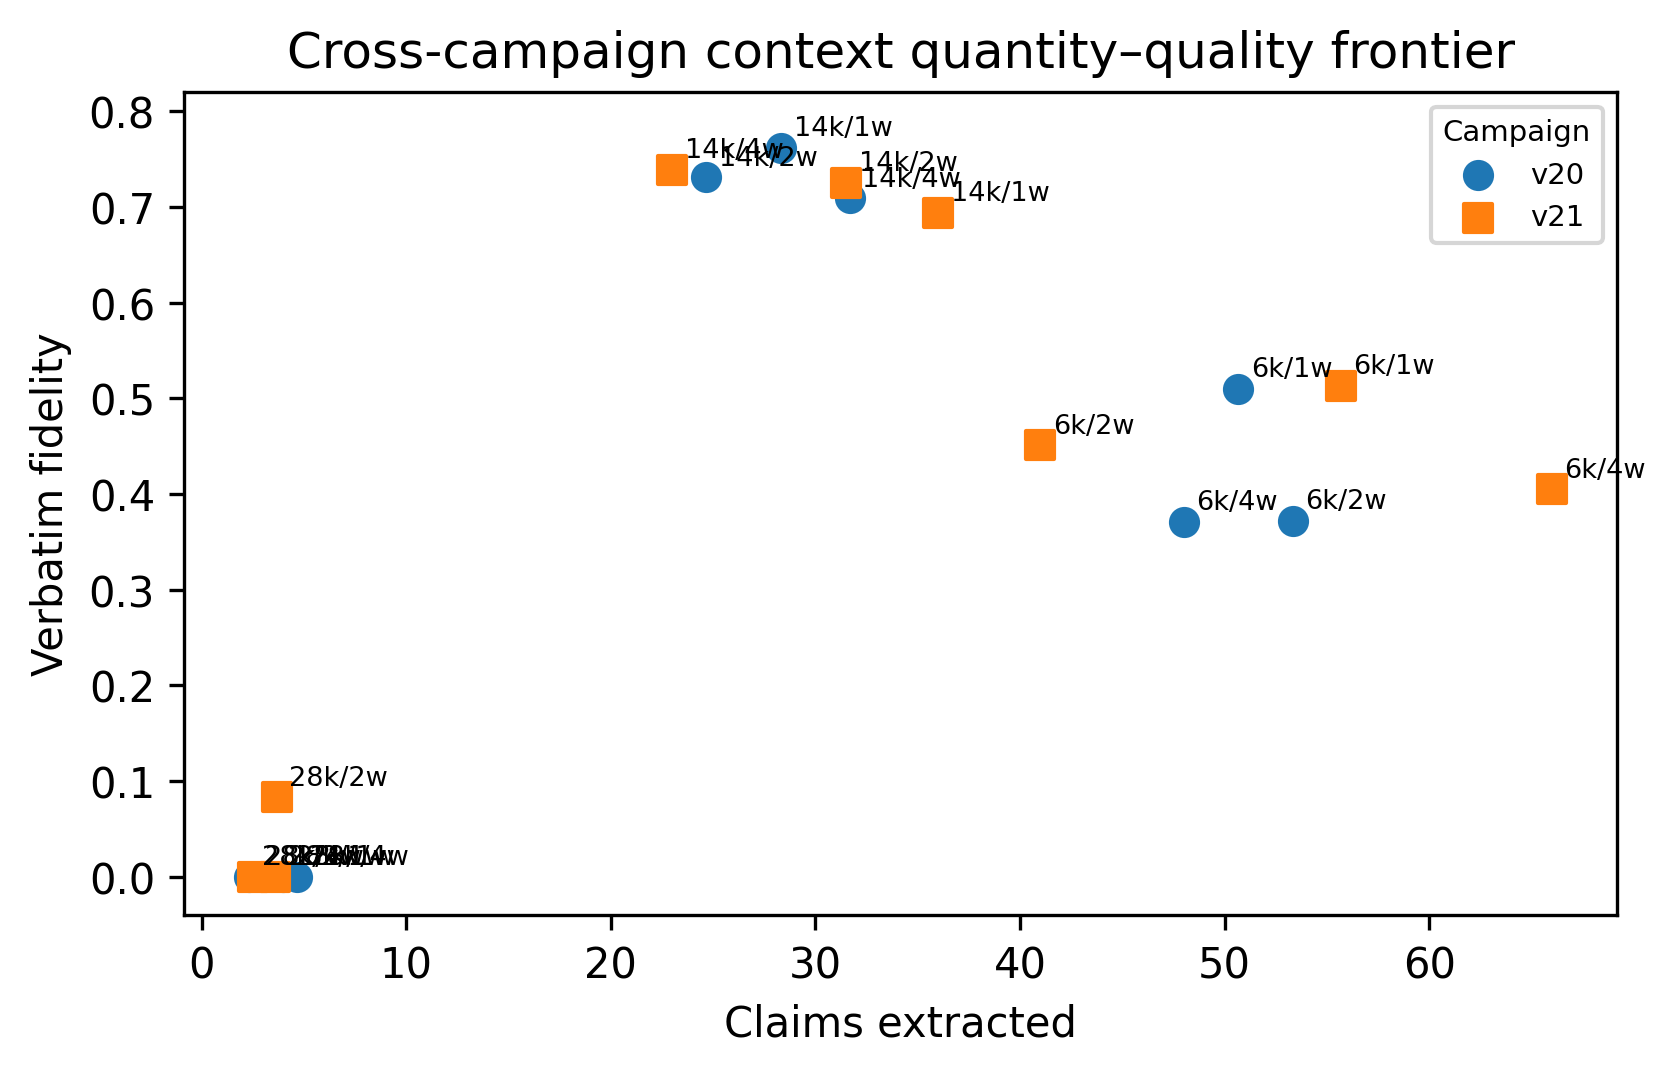
\includegraphics[width=\columnwidth]{figures/fig_context_frontier.png}
\caption{Cross-campaign context frontier. Each point is a window--worker cell; the repeated separation between 6k (higher quantity), 14k (higher fidelity), and 28k (near-collapse) is more informative than any single wall-clock optimum.}
\label{fig:context-frontier}
\end{figure}

The \emph{quality} ordering replicates; the efficiency ordering does not. Applying Eq.~\ref{eq:utility} to campaign~B places its best 6k cell at 19.90\,s per verified claim against 29.75\,s for 14k with one worker---the reverse of campaign~A. The cause is the endpoint outage described in Section~IV-A, not anything about context size. It covered the final 65 minutes of a 207-minute campaign and, because cells execute in randomised order, removed attempts from eight of the nine cells; the 14k single- and four-worker cells were each left with one successful run. An outage is independent of the factor under test, so the survivors are not biased toward a configuration---there are simply too few of them, and at $n=1$ a cell mean is a single observation. We therefore report $E_v$ from the failure-free campaign and treat cross-campaign agreement on \emph{orderings} of quantity and fidelity, rather than on efficiency magnitudes, as the replicable result.

The partition arithmetic clarifies the mechanism. The source document yields six windows at 6k, three at 14k and two at 28k, and mean calls per run track that split closely (33.7, 18.7 and 2.3 in campaign~A). The 28k regime is thus not a long-context model failing to attend to a long input so much as an agent configuration that reduces the task to two very large requests, each of which must emit a long structured array in a single generation. The observable consequence is that the quotations it returns do not appear in the source at all. Several 28k cells finish quickly precisely because they produce little verified content; Eq.~\ref{eq:utility} rejects this false optimum by normalising resource use by verified extraction, as Table~\ref{tab:ev} shows directly.

\subsection{RQ2: Model size is not a sufficient capacity proxy}
\label{sec:models}
Table~\ref{tab:models} reports model operating points observed under specific extraction workloads, provider configurations and execution periods. These are not exchangeable repetitions: differences in model family, training objective, serving backend and provider load can influence both quality and latency. The reported rankings are conditional on the evaluated workload and environment, not general-purpose model rankings.

In the earlier campaign's same-task comparison, the general-purpose 8B model is 7.32$\times$ faster than the 70B (113.72 against 832.16\,s), extracts 1.59$\times$ as many claims, and requires 4.03 rather than 51.44 seconds per verified claim---a 12.77$\times$ efficiency advantage. The later campaign broadens the family: a 31B calibrated/general model attains the highest fidelity (.726) and stability (.845), while a 550B/A55B reasoning model is faster but markedly less source-grounded (.404). Here \emph{lightweight} denotes a relatively small parameter count, exemplified by the 8B endpoints, rather than a measured low-memory or low-power deployment; actual memory, throughput and latency also depend on quantisation, context length, architecture, batching and hardware.

The safety-specialised 8B endpoint failed all three attempts, and the mechanism is instructive. It did not refuse, time out or return an HTTP error: it returned status 200 with syntactically valid JSON---\texttt{\{"User Safety": "safe", "Response Safety": "safe"\}}---the schema of its own content-classification task rather than the requested extraction schema. The extraction contract is deliberately permissive, accepting a bare array, four alternative wrapper names, or a single unwrapped claim, so this was not a formatting near-miss that a stricter parser created; it was a different answer to a different question. Schema repair reissued the request and received an elaborated version of the same object; validation failed, the affected windows yielded no claims, and the run terminated after a mean 19.3\,s (sd 3.4). Every layer that could have caught this reported success---transport, JSON parser and the provider's own structured-output path---and only application-side schema validation rejected it. Parameter count is thus not merely an imperfect capability proxy: it does not encode the model's task contract at all, and OpenAI-compatible request syntax does not guarantee response-semantic compatibility.

\begin{table*}[t]
\caption{Model/role operating points across campaigns. Means over successful runs; sd is the sample standard deviation of wall time. Failed cells are retained as deployment evidence rather than assigned artificial quality scores.}
\label{tab:models}
\centering\scriptsize
\begin{tabular}{llrrrrrrr}
\toprule
Campaign & Model role/capacity & Success & Time(s) & sd & Claims & $V$ & Stability & s/verified\\
\midrule
A & Llama-3.1 8B instruction & 5/5 & 113.72 & 37.7 & 58.2 & .485 & .348 & 4.03\\
A & Llama-3.3 70B instruction & 5/5 & 832.16 & 256.6 & 36.6 & .442 & .552 & 51.44\\
B & 31B calibrated/general & 3/3 & 491.77 & 253.4 & 25.3 & \textbf{.726} & \textbf{.845} & 26.74\\
B & 550B/A55B reasoning & 3/3 & 306.50 & 74.8 & 17.3 & .404 & .796 & 43.77\\
B & 8B safety-specialised & 0/3 & 19.27$^*$ & 3.4 & -- & -- & -- & --\\
\bottomrule
\multicolumn{9}{l}{\scriptsize $^*$Mean elapsed time until unsuccessful termination; no valid extraction was produced.}
\end{tabular}
\end{table*}

\subsection{RQ3: Moderate fan-out is robust; maximum fan-out is not}
\emph{Fan-out} denotes the number of agent workers permitted to dispatch model requests concurrently. It controls application-level request concurrency, not the number of GPUs or the serving engine's internal batch size. The agent fans out at two distinct stages, over two different units of work, and the distinction turns out to govern the result:

\begin{itemize}
\item \textbf{Extraction} maps over \emph{document windows}: the 34{,}651-character source at a 14k window gives three windows, dispatched over $\min(2,c)$ workers---capped at two because extraction issues the longest generations and was the stage most prone to timeout.
\item \textbf{Verification} maps over \emph{individual claims}---one reference lookup and one groundedness check each---over all $c$ workers. A representative run extracts 40 claims across 40 distinct references: at $c=1$ one worker performs all 40 checks; at $c=2$, about 20 each; at $c=4$, about 10 each.
\end{itemize}

Consequently $c=2$ and $c=4$ are \emph{identical} in the extraction stage and differ only in verification. Moving from one worker to two shortens both stages; moving from two to four shortens neither extraction nor the per-claim work, and merely raises instantaneous request pressure on the endpoint.

The measurements match that structure. Table~\ref{tab:fanout} shows the lowest mean wall time at $c=2$ in both campaigns. Relative to one worker, two workers reduce mean time by 39.3\% in campaign~A and 3.9\% in campaign~B; four workers are slower than two in both, and slower than one in campaign~B. The finding is strengthened by the substrate difference: campaign~A ran on the hosted OpenAI-compatible endpoint and campaign~B entirely on the local single-user runtime, so the two-worker optimum replicates across serving designs with very different concurrency models, even though absolute latencies and the size of the gain do not transfer. Residual effects beyond the stage structure are compatible with server-side queueing, batching, KV-cache pressure or scheduler contention; the available telemetry does not permit attribution to a single mechanism. Modern inference servers explicitly schedule concurrent and in-flight requests, so client-side workers cannot be assumed to map linearly to independent compute \cite{yu2022orca,agrawal2024sarathi,nvidiaDynamoPlanner}.

\begin{table}[t]
\caption{Fan-out replication across two serving substrates. Means over successful runs only ($n$ shown).}
\label{tab:fanout}
\centering\scriptsize
\begin{tabular}{llrrrrr}
\toprule
Campaign & Workers & $n$ & Time(s) & sd & $V$ & s/verified\\
\midrule
A (hosted) & 1 & 5 & 495.56 & 91.0 & .334 & 43.13\\
A (hosted) & \textbf{2} & 4 & \textbf{300.85} & 54.6 & .392 & \textbf{21.03}\\
A (hosted) & 4 & 5 & 384.06 & 179.5 & .363 & 32.26\\
\midrule
B (local) & 1 & 5 & 736.58 & 35.4 & .325 & 125.91\\
B (local) & \textbf{2} & 4 & \textbf{707.70} & 122.6 & .419 & \textbf{112.60}\\
B (local) & 4 & 5 & 920.08 & 383.4 & .452 & 127.22\\
\bottomrule
\end{tabular}
\end{table}

\subsection{Coordination depth}
The protocol campaign varies critic rounds in a rubric-based assessment agent rather than the extraction agent, and its figures are therefore not directly comparable with the preceding sections. Increasing critic rounds from one to two raises pooled recall from .341 to .353, corroboration from .827 to .967 and stability from .374 to .552. A third round preserves recall and corroboration but does not improve stability (.537). Mean wall time is not monotonic (189.4, 179.9 and 140.7\,s for one, two and three rounds, with sd 37.5, 92.0 and 58.2), reinforcing that hosted wall time is a system observation influenced by scheduling and service state rather than a count of logical reasoning steps. The practical reading is that the second critic round buys most of the available agreement and the third buys none.

\section{Discussion}
\subsection{Best practice: optimise a frontier, not a knob}
The experiments reject three tempting heuristics: ``use the longest context'', ``use the largest model'' and ``add more workers''. Each selects a dominated operating point in at least one campaign. A safer procedure is: (i) fix $V_{\min}$ from the downstream task before tuning; (ii) sweep a small set of context, role and concurrency choices---nine cells sufficed in Table~\ref{tab:ev}; (iii) record realised rather than configured serving identity; (iv) estimate CCR components and, where telemetry allows, TTFT/ITL; and (v) choose the Pareto point minimising seconds or cost per verified output. Where monetary rather than latency cost dominates, $T$ in Eq.~\ref{eq:utility} can be replaced by $(N_{in}/10^6)\pi_{in}+(N_{out}/10^6)\pi_{out}$ for provider unit prices $\pi$, leaving the method unchanged.

The context result is the most consequential. Long context can increase capability, but partitioning determines both the statistical task presented to the model and the workload presented to the server: a larger partition raises prefill work and KV state while changing extraction density and attention competition. The repeated 28k regime shows that a fast response can be a low-utility response, so throughput metrics should be paired with task-grounded yield---verified claims per second, not tokens per second alone.

\subsection{CCR as an online partition controller}
CCR bridges classical distributed partitioning and agent inference. When $CCR_{PD}$ is high, fixed invocation and communication dominate and overly fine partitioning wastes resources: prefer larger chunks or batching. When it is low, token processing dominates and finer partitions may reduce prefill/decode work, provided they retain sufficient context. Our measurements place 6k on the overhead-dominated side and 28k on the degenerate-quality side, with 14k between them---precisely the regime a controller should seek. Because effective $t_p$, $t_d$ and $\epsilon$ depend on provider load, hardware, batching and concurrency, they require per-environment calibration; the present campaigns establish application-level operating points, and phase-specific coefficient estimation remains conditional on suitable telemetry. NVIDIA's profiler follows the same principle, interpolating TTFT against input length and ITL against KV usage \cite{nvidiaDynamoProfiler}. The step proposed here is to couple those fitted costs to extraction quality through Eq.~\ref{eq:utility}.

\subsection{Interoperability requires semantic and telemetry standards}
OpenAI-compatible request syntax is valuable, but our campaigns show why portability needs a stronger contract. The safety-specialised endpoint in Section~\ref{sec:models} satisfied every syntactic expectation and still could not perform the role assigned to it, and the 96 mid-run fallbacks in Section~\ref{sec:context} would have been invisible to any analysis trusting the configured model. The minimum interoperable record for an agent call should expose: immutable provider and model/revision identity; input and output token counts; TTFT and ITL/TPOT where streaming is available; queue and server-processing time where available; structured-output and finish status; retry/fallback lineage; and a stable error taxonomy. Without these fields, two ``compatible'' endpoints can execute the same logical agent while leaving different evidence for optimisation and audit.

We therefore advocate a lightweight \emph{LLM Inference Trace}, analogous in spirit to portable model formats and observability standards: API syntax remains provider-specific or OpenAI-compatible, while a common sidecar schema records execution semantics. Such a standard would let campaign files survive catalogue evolution, permit hosted and local runs to coexist in one analysis---as fan-out campaigns A and B do here---and enable fair comparison without pretending the environments are identical. It also benefits providers: richer telemetry makes queueing, batching and phase-specific performance visible to application optimisers instead of being misattributed to model quality.

\subsection{How to generalise without erasing variation}
Generalisation does not require discarding configurations; it requires preserving the dimensions along which they differ. We therefore distinguish \emph{within-campaign causal contrasts} from \emph{cross-campaign replicated orderings}. The 8B/70B comparison is a within-campaign model-choice contrast, though serving conditions and architecture may still confound a parameter-count reading; the 8B/31B/550B campaign extends the envelope but changes model family and objective. Their joint implication is not a universal ranking of parameter counts but the more portable conclusion that parameter count alone is insufficient for role assignment. Likewise, absolute fan-out latency differs sharply between campaigns A and B, yet the two-worker optimum replicates across both substrates. This ``retain, label, replicate'' strategy is preferable to discarding evidence whenever a catalogue changes.

\section{Limitations and Threats to Validity}
The study is an application-level systems evaluation, not a controlled GPU microbenchmark. Hosted endpoints expose only part of the serving state; hardware allocation, batching, queue depth, quantisation and co-tenant load vary over time. We therefore avoid attributing wall-clock differences to any single internal mechanism and model unobserved state through $\epsilon$. Provider and model differences across campaigns also preclude a single pooled causal estimate of parameter-count effects; we report labelled operating points and replicated orderings.

The automated fidelity metrics assess source-text correspondence rather than semantic correctness or completeness. No independently annotated human subset is reported here, so the findings establish a frontier for automated source-grounded extraction quality, not for human-judged factual accuracy; establishing the correspondence between the two requires human assessment of correctness, context preservation and missed claims.

Repetitions per condition are modest and unequal, and the cross-condition ranges in Table~\ref{tab:context} do not quantify sampling uncertainty. Where failures concentrated, some cells rest on a single successful run, so their standard deviations are zero by construction rather than by precision. Per-cell standard deviations are reported where $n>1$; bootstrap or confidence intervals over additional repetitions would improve precision assessment. Replicated qualitative trends should not be read as established population effects, and further runs across independent workloads, hardware and providers remain necessary for generality.

Finally, the experiments cover one agent architecture and two task families. The proposed schema and CCR method are generic, but optimal thresholds require workload-specific calibration. These limitations are themselves a systems finding: providers increasingly expose TTFT/ITL and phase-aware planning because application performance cannot be inferred from model name and token count alone \cite{nvidiaDynamoPlanner,mlperf2025llm}. Wider adoption of standard per-request telemetry would let future studies separate application, network, queue, prefill and decode effects precisely.

\section{Conclusion}
Across 136 attempted runs and 1{,}689 realised model calls, LLM-agent extraction shows stable resource--quality structure despite changing model and serving conditions. Medium context dominates maximum context for source-grounded fidelity in both partitioning campaigns, and minimises seconds per verified claim in the campaign measured without failures; two-way fan-out gives the best latency on two different serving substrates; and parameter count does not monotonically predict extraction utility, with one endpoint returning valid JSON of entirely the wrong schema. These findings argue for workload-calibrated operating points rather than maximum-size configurations.

We extend the communication--computation ratio to a prefill/decode-aware $CCR_{PD}$ and combine it with verified-output efficiency to guide context selection, demonstrating the rule on measured cells. More broadly, portable agent optimisation requires preserving realised model/provider identity and standardising phase-specific telemetry, retry/fallback provenance and output semantics. The goal is not to eliminate provider diversity but to make heterogeneous hosted and local inference measurable through one systems contract.

\balance
\bibliographystyle{IEEEtran}
\bibliography{references}
\end{document}
